\subsection{Experimental Design} \label{sec:expDesign}
  Our evaluation is based on two benchmarks with significantly different access
  patterns. The first is quicksort (Qsort). This benchmark first allocates a
  large array of random numbers, and then sorts it using the well-known
  quicksort algorithm.  Quicksort is a divide and conquor algorithm that
  automatically partitions the input array into small local blocks before
  performing a final sort. This leads to excellent cache behavior and
  predictible access patterns.  Furthermore, by allocating the input array
  dynamically, quicksort performs no file I/O, so it is never blocked on I/O or
  other OS interactions.

  The other benchmark is a de-novo genome assembly benchmark (Gen). Gen begins
  by loading a large text file that represents raw genome data. Raw genome data
  consists of short, overlapping, sequences of base-pairs called "contigs", the
  goal is to align these overlapping contigs into a single contiguous sequence
  representing a genome. This is done by loading contigs into a large hash
  table and probing into it repeatedly to find matching sequences. This leads
  to very little locality and unpredictible access patterns. Furthermore, Gen
  performs file I/O on the input, which allows for more complex OS
  interactions.

\subsection{End-to-End Performance} \label{sec:fullPerf}
  The benchmarks were both run under a cgroup in Linux in order to reduce the
  available memory and emulate a system with low local memory. In this
  experiment, we disable kpfad in order to isolate the batching of new-page
  management from the scheduling flexibility offered by kswapd's asynchrony.
  The PFA was configured to allow up to 64 outstanding page faults before
  bookkeeping was performed.

  \begin{figure}[h] \centering
    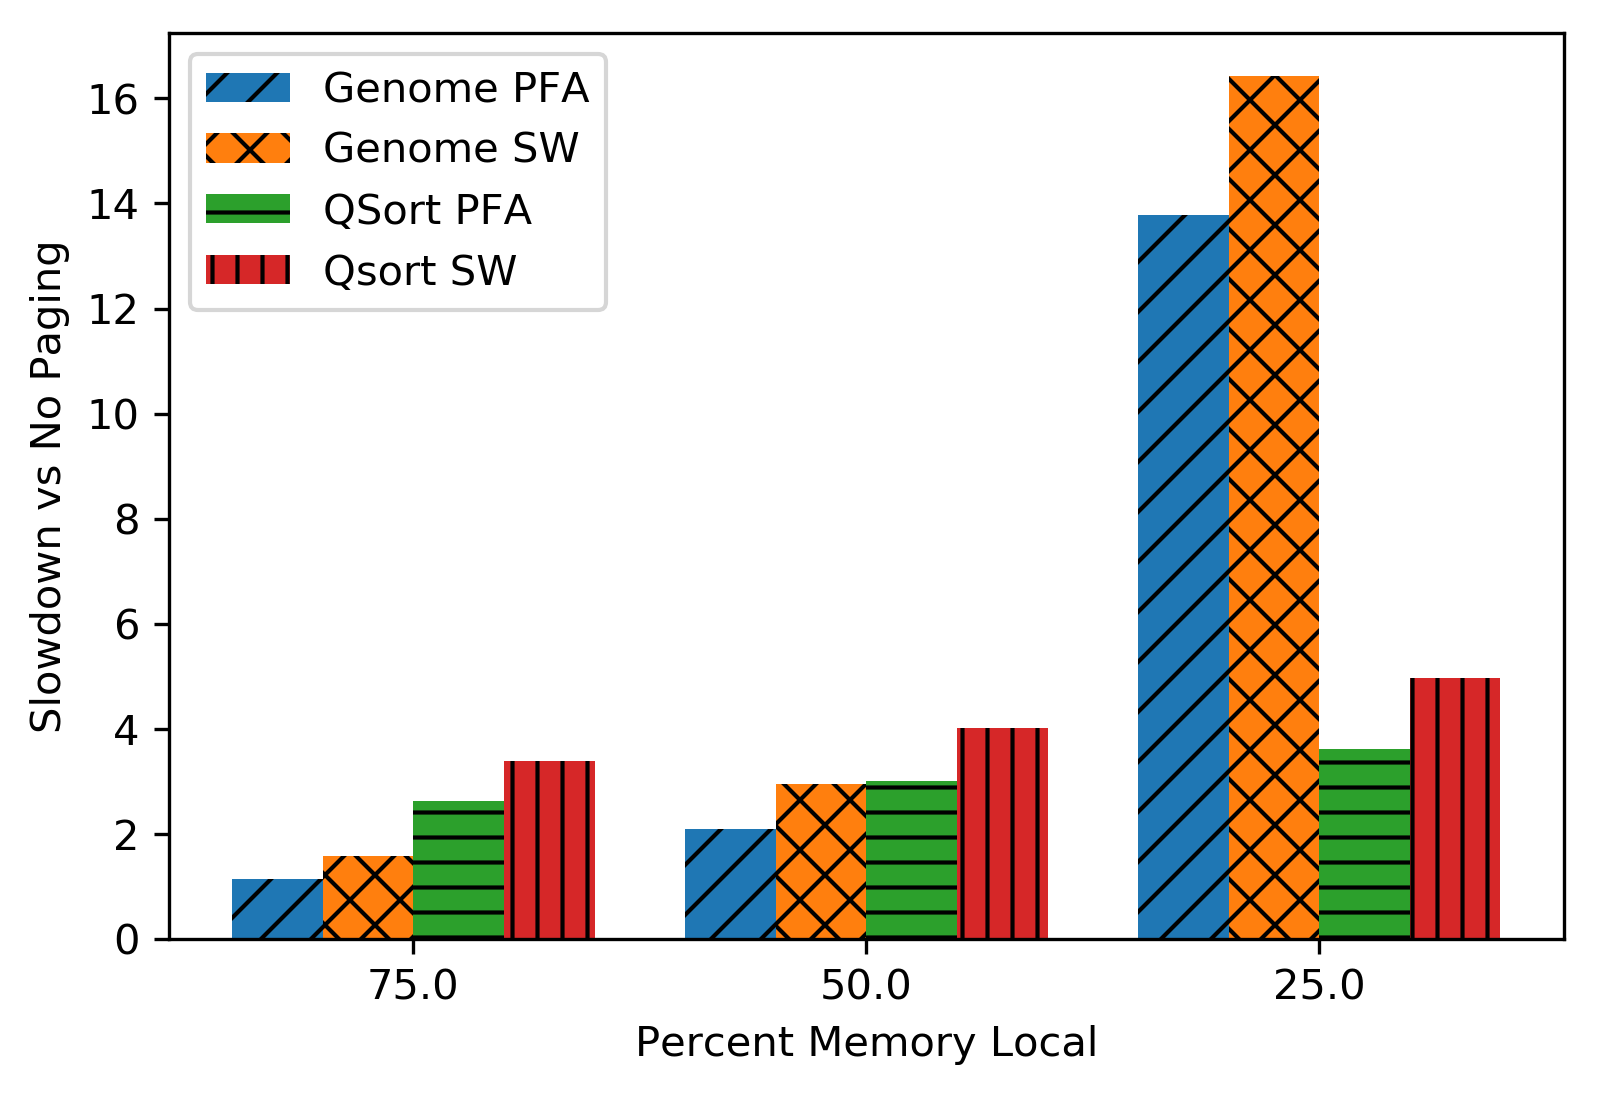
\includegraphics[width=0.9\columnwidth]{figs/pfa_perf_nokswapd.png}
    \vspace{-5mm}
    \caption{PFA vs Baseline without kswapd}
    \label{fig:pfa_perf}
  \end{figure}

  Both applications were tuned to use 64MB of memory at their peak. We then
  varied the cgroup memory limit from 100\% (64MB) down to 25\% (16MB),
  triggering increasing levels of paging. For both benchmarks, the PFA
  significantly reduces the overhead (by up to 1.4x). A more detailed analysis
  shows that while the number of evicted pages is the same in both
  configurations, using the PFA leads to a 2.5x reduction in metadata
  management time on average. While the same code path is executed for each new
  page, the PFA batches these events, leading to improved cache locality for
  the OS, and fewer cache-polluting page-faults for the application.

